\subsection{Системы типов и \texorpdfstring{$\lambda$}{лямбда}-исчисление}

В основе систем автоматического доказательства теорем, как правило, лежит вычислительнный формализм, известный как $\lambda$-исчисление. Это формальная система, придуманная в 30-ых годах прошлого века Алонзо Черчём(англ. Alonso Church)~\cite{church1936unsolvable} с целью анализа и формализации понятия вычислимости. В 60-ых годах Питером Ландином(англ. Peter Landin) была опубликована работа~\cite{landin1964mechanical}, в которой выдвигалась идея о том, что $\lambda$-исчисление может использоваться для моделирования различных выражений в языках программирования того времени, что в дальнейшем привело к развитию языков в стиле \textbf{ML}. С тех пор идеи $\lambda$-исчисления широко используются в мире функционального программирования.

Формально, $\lambda$-термы определяются индуктивно, следующим образом:

\begin{enumerate}
  \item Если $x$ -- переменная, то $x$ -- $\lambda$-терм.
  \item Если $M$ и $N$ -- $\lambda$-термы, то $M\ N$ -- тоже $\lambda$-терм.
  \item Если $x$ -- переменная, а $M$ -- $\lambda$-терм, то $\lambda x.M$ -- тоже $\lambda$-терм.
\end{enumerate}

Изначально, в $\lambda$-исчислении не вводилось никаких правил типизации(встречается термин <<бестиповое>> или <<чистое>> $\lambda$-исчисление, англ. untyped $\lambda$-calculus), однако в дальнейшем появилось множество типизированных вариаций. Хенком Барендрегтом(нидерл. Hendrik Pieter Barendregt) в~\cite{barendregt1993lambda} описан так называемый $\lambda$-куб, который наглядно классифицирует восемь различных систем типизации лямбда-исчисления.

\begin{figure}[H]
  \centering
  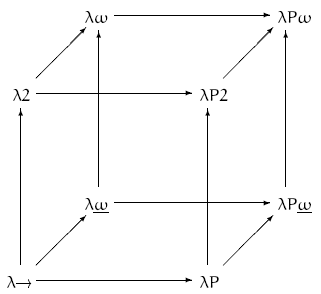
\includegraphics[width=0.5\textwidth]{img/Lambda_cube.png}
  \caption{Лямбда-куб\protect\footnotemark}
\end{figure}

\footnotetext{Изображение взято с сайта \url{https://en.wikipedia.org/wiki/Lambda_cube}, автор -- Денис Москвин}

База куба -- просто типизированное $\lambda$-исчисление($\lambda{\to}$), в котором термы могут зависеть только от термов. Три оси соответствуют расширениям, комбинации которых позволяют получить остальные системы типов:

\begin{enumerate}
  \item Термы, которые зависят от типов -- система $\lambda2$ или \textbf{System F}
  \item Типы, которые зависят от типов -- система $\lambda \underline{\omega}$(операторы над типами)
  \item Типы, которые зависят от термов -- система $\lambda P$(зависимые типы)
\end{enumerate}

Нам не очень сейчас важно, каким образом устроены конкретные системы типов. Вместо этого, мы обсудим, какое отношение они имеют к доказателям теорем.

Соответствие Карри-Говарда~\cite{howard1980formulae} устанавливает прямую связь между логикой и теорией типов. Логической связке соответствует конструкция в теории типов, а логическому утверждению -- тип. Доказательству того факта, что утверждение истинно, соответствует тогда доказательство того факта, что соответствующий этому утверждению тип населен. То есть для доказательства утверждений мы можем писать программы на языке $\lambda$-исчисления, имеющие требуемый тип, тогда при проверке типов специальный компонент проверит, является ли наше доказательство корректным по отношению к исходному утверждению.

Незамедлительно становится ясно, что чем больше конструкций в своем распоряжений мы имеем в системе типов, тем более большой класс утверждений мы можем доказывать. Например, система автоматического доказательства теорем \textbf{Coq} основана на так называемом исчислении конструкций, соответствующему вершине $\lambda{}P{}\omega$ лямбда-куба.

Кроме этого, становится ясно, какие ограничения есть у доказателей теорем. Поскольку мы хотим выводить и проверять, является ли доказательство корректным, то нам хочется, что бы проверка типов в нашем языке всегда завершалась за конечное число шагов -- иначе говоря, была разрешимой. На этапе проверки типов может происходить вычисление значений функций, которые мы определеии в нашем языке. Как следствие, от функций, которые мы определяем в нашей теории требуется, что бы они были определены для всех значений входных параметров(то есть быть тотальными).
